\documentclass[french]{article}
\usepackage[T1]{fontenc}
\usepackage[utf8]{inputenc}
\usepackage{lipsum}
\usepackage{lmodern}
\usepackage{geometry}
\usepackage{babel}
\usepackage{graphicx}
\usepackage{lastpage}
\usepackage{ragged2e}
\usepackage{enumitem}
\usepackage[normalem]{ulem}
\usepackage{hyperref} % pour \url{URL}
\usepackage{color} % pour \textcolor{color}{text}
\usepackage{listings} % pour afficher du code
\usepackage{longtable} % pour l'environnement longtable
\usepackage{float} % pour des figures non flottantes
\usepackage{amsmath}
\usepackage{verbatim} % pour les graphes
\usepackage{caption} % figure et subfigure pour mettre les images côtes à côtes
\usepackage{subcaption}
\usepackage{dirtree}
\usepackage{pdfpages}
% Pdf
\setboolean{@twoside}{false}

% Grammaire EBNF
\usepackage{syntax}
\setlength{\grammarparsep}{5pt plus 1pt minus 1pt}
\setlength{\grammarindent}{11em}

% Dessin avec tikz
\usepackage{tikz}
\usetikzlibrary{shapes,arrows,positioning,shadows,matrix,automata}

% Matrices
\usepackage{kbordermatrix}% http://www.hss.caltech.edu/~kcb/TeX/kbordermatrix.sty

% Largeur de colonnes de tableau fixes
\usepackage{array}
\newcolumntype{L}[1]{>{\raggedright\let\newline\\\arraybackslash\hspace{0pt}}m{#1}}
\newcolumntype{C}[1]{>{\centering\let\newline\\\arraybackslash\hspace{0pt}}m{#1}}
\newcolumntype{R}[1]{>{\raggedleft\let\newline\\\arraybackslash\hspace{0pt}}m{#1}}


% CSS
\lstdefinelanguage{CSS}{
	keywords={color,background-image:,margin,padding,font,weight,display,position,top,left,right,bottom,list,style,border,size,white,space,min,width, transition:, transform:, transition-property, transition-duration, transition-timing-function},	
	sensitive=true,
	morecomment=[l]{//},
	morecomment=[s]{/*}{*/},
	morestring=[b]',
	morestring=[b]",
	alsoletter={:},
	alsodigit={-}
}

% JavaScript
\lstdefinelanguage{JavaScript}{
	morekeywords={typeof, new, true, false, catch, function, return, null, catch, switch, var, if, in, while, do, else, case, break, let},
	morecomment=[s]{/*}{*/},
	morecomment=[l]//,
	morestring=[b]",
	morestring=[b]',
	morestring=[s]{/[}{/;}
}

\lstdefinelanguage{HTML5}{
	language=html,
	sensitive=true,	
	alsoletter={<>=-},	
	morecomment=[s]{<!-}{-->},
	tag=[s],
	otherkeywords={
		% General
		>,
		% Standard tags
		<!DOCTYPE,
		</html, <html, <head, <title, </title, <style, </style, <link, </head, <meta, />,
		% body
		</body, <body,
		% Divs
		</div, <div, </div>, 
		% Paragraphs
		</p, <p, </p>,
		% scripts
		</script, <script,
		% More tags...
		<canvas, /canvas>, <svg, <rect, <animateTransform, </rect>, </svg>, <video, <source, <iframe, </iframe>, </video>, <image, </image>, <header, </header, <article, </article
	},
	ndkeywords={
		% General
		=,
		% HTML attributes
		charset=, src=, id=, width=, height=, style=, type=, rel=, href=,
		% SVG attributes
		fill=, attributeName=, begin=, dur=, from=, to=, poster=, controls=, x=, y=, repeatCount=, xlink:href=,
		% properties
		margin:, padding:, background-image:, border:, top:, left:, position:, width:, height:, margin-top:, margin-bottom:, font-size:, line-height:,
		% CSS3 properties
		transform:, -moz-transform:, -webkit-transform:,
		animation:, -webkit-animation:,
		transition:,  transition-duration:, transition-property:, transition-timing-function:,
	}
}

\lstdefinestyle{htmlcssjs} {%
	% General design
	%  backgroundcolor=\color{editorGray},
	basicstyle={\footnotesize\ttfamily},   
	frame=b,
	% line-numbers
	xleftmargin={0.75cm},
	numbers=left,
	stepnumber=1,
	firstnumber=1,
	numberfirstline=true,	
	% Code design
	identifierstyle=\color{black},
	keywordstyle=\color{blue}\bfseries,
	ndkeywordstyle=\color{black}\bfseries,
	stringstyle=\color{brown}\ttfamily,
	commentstyle=\color{gray}\ttfamily,
	% Code
	language=HTML5,
	alsolanguage=JavaScript,
	alsodigit={.:;},	
	tabsize=2,
	showtabs=false,
	showspaces=false,
	showstringspaces=false,
	extendedchars=true,
	breaklines=true,
	% German umlauts
	literate=%
	{Ö}{{\"O}}1
	{Ä}{{\"A}}1
	{Ü}{{\"U}}1
	{ß}{{\ss}}1
	{ü}{{\"u}}1
	{ä}{{\"a}}1
	{ö}{{\"o}}1
}
%
\lstdefinestyle{py} {%
	language=python,
	literate=%
	*{0}{{{\color{lightred}0}}}1
	{1}{{{\color{lightred}1}}}1
	{2}{{{\color{lightred}2}}}1
	{3}{{{\color{lightred}3}}}1
	{4}{{{\color{lightred}4}}}1
	{5}{{{\color{lightred}5}}}1
	{6}{{{\color{lightred}6}}}1
	{7}{{{\color{lightred}7}}}1
	{8}{{{\color{lightred}8}}}1
	{9}{{{\color{lightred}9}}}1,
	basicstyle=\footnotesize\ttfamily, % Standardschrift
	numbers=left,               % Ort der Zeilennummern
	%numberstyle=\tiny,          % Stil der Zeilennummern
	%stepnumber=2,               % Abstand zwischen den Zeilennummern
	numbersep=5pt,              % Abstand der Nummern zum Text
	tabsize=4,                  % Groesse von Tabs
	extendedchars=true,         %
	breaklines=true,            % Zeilen werden Umgebrochen
	keywordstyle=\color{blue}\bfseries,
	frame=b,
	commentstyle=\color{gray}\itshape,
	stringstyle=\color{brown}\ttfamily, % Farbe der String
	showspaces=false,           % Leerzeichen anzeigen ?
	showtabs=false,             % Tabs anzeigen ?
	xleftmargin=17pt,
	framexleftmargin=17pt,
	framexrightmargin=5pt,
	framexbottommargin=4pt,
	%backgroundcolor=\color{lightgray},
	showstringspaces=false,      % Leerzeichen in Strings anzeigen ?
}%

\geometry{
	a4paper,
	total={210mm,297mm},
	left=20mm,
	right=20mm,
	top=20mm,
	bottom=20mm,
}

\usepackage{fancyhdr}
\pagestyle{fancy}
\setlist[enumerate,1]{leftmargin=2cm}

% Entêtes
\lhead{Champion, Loiseau\\Rochat, Schubert}
\chead{}
\rhead{PDG: Manuel utilisateur}
\renewcommand{\headrulewidth}{0.4pt}
\renewcommand{\footrulewidth}{0.4pt}

\begin{document}
	
	
	% Titre du document
	\title{Projet Rady} % ou un autre nom\centering
	\author{Manuel de l'utilisateur\\ 
		Projet de groupe\\
		Champion, Loiseau, Rochat, Schubert\\
		Resp. René Rentsch\\
		HEIG-VD}
	\date{\today} % date du jour
	\maketitle
	\vspace{2cm}
	\centering
	
\includegraphics[scale=0.3]{../logo/icone}
	\thispagestyle{empty}
	
	\newpage
	\thispagestyle{empty}
	$ $
	\newpage
	
	% Pour tout le document
	\justify
	\normalsize
	
	% Tables des matières
	\tableofcontents
	
	\newpage	
	\section{Introduction}
	Bienvenue dans ce manuel de l’utilisateur l'application mobile Rady. Ce manuel est à destination des nouveaux utilisateurs. Nous espérons que les explications que vous y trouverez concernant chaque interface vous seront pleinement profitable. Nous vous souhaitons une excellente visite de notre application.  
	
	\bigskip
	\bigskip
	
	Cordialement.
	\newline
	L'équipe de développement Rady.
		
	\section{Installation}
	
	Pour une installation facile, veuillez vous rendre avec votre smartphone android sur :
	\bigskip
	
	\centering
	https://rady.benschubert.me/login?redirect=stats
	
	\bigskip
	\justifying 
	Puis cliquez sur Download App. L'apk doit maintenant se télécharger sur votre appareil. Une fois cela fini vous devriez avoir un popup qui apparait dans le bas de votre écran. Veuillez alors cliquer sur ouvrir.
	Dès ce moment la l'installation devrait se lancer.
	\newline
	\newline
	
	Si l'installation n'a pas eu lieu et que vous recevez un message d'erreur vous indiquant que l'installation est bloqué, vous devrez accéder aux paramètres, accepter les installations provenant de sources inconnues et valider. Dès lors vous devriez pouvoir installer.
	
	
	
	\section{Interfaces}
	\subsection{Sign-in}
	\begin{figure}[H]
		\centering
		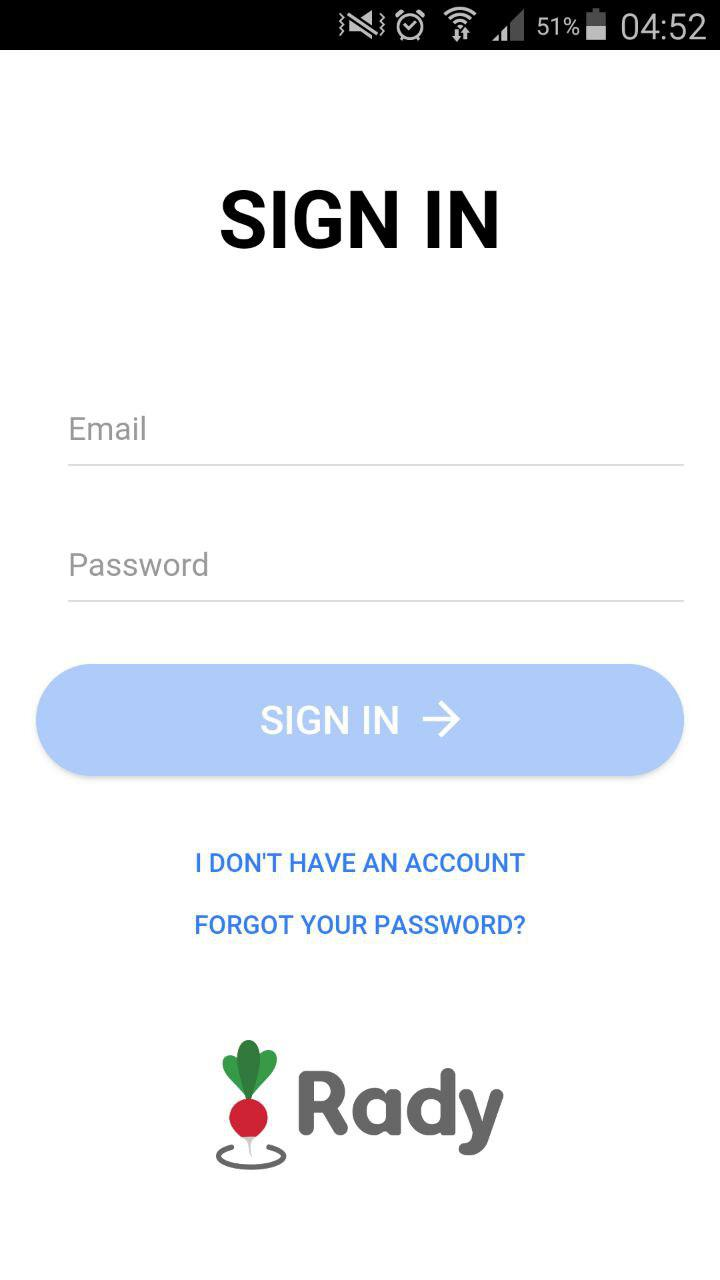
\includegraphics[scale=0.4]{../screenshot/screenshot-sign-in}
		\caption{Sign-in}
		\label{Sign-in}
	\end{figure} 
	
	Voici la première interface sur laquelle vous devriez arriver au lancement de l'application. Sur cette page vous pouvez vous authentifier pour l'application à l'aide de votre mot de passe et de votre e-mail, si vous avez déjà créer un compte. Si vous ne possédez pas de compte alors veuillez cliquer sur :
	\bigskip
	
	\centering
	I DON'T HAVE AN ACCOUNT
	
	\bigskip
	\justifying 
	Celà vous mènera à la page Register.
	\newline
	Si vous avez oublié votre mot de passe vous pourrez obtenir l'aide d'un gestionaire de récupération de mot de passe en cliquant sur :
	\bigskip
	
	\centering
	FORGOT YOUR PASSWORD
	
	\bigskip
	\justifying 
	\subsection{Register}
	\begin{figure}[H]
		\centering
		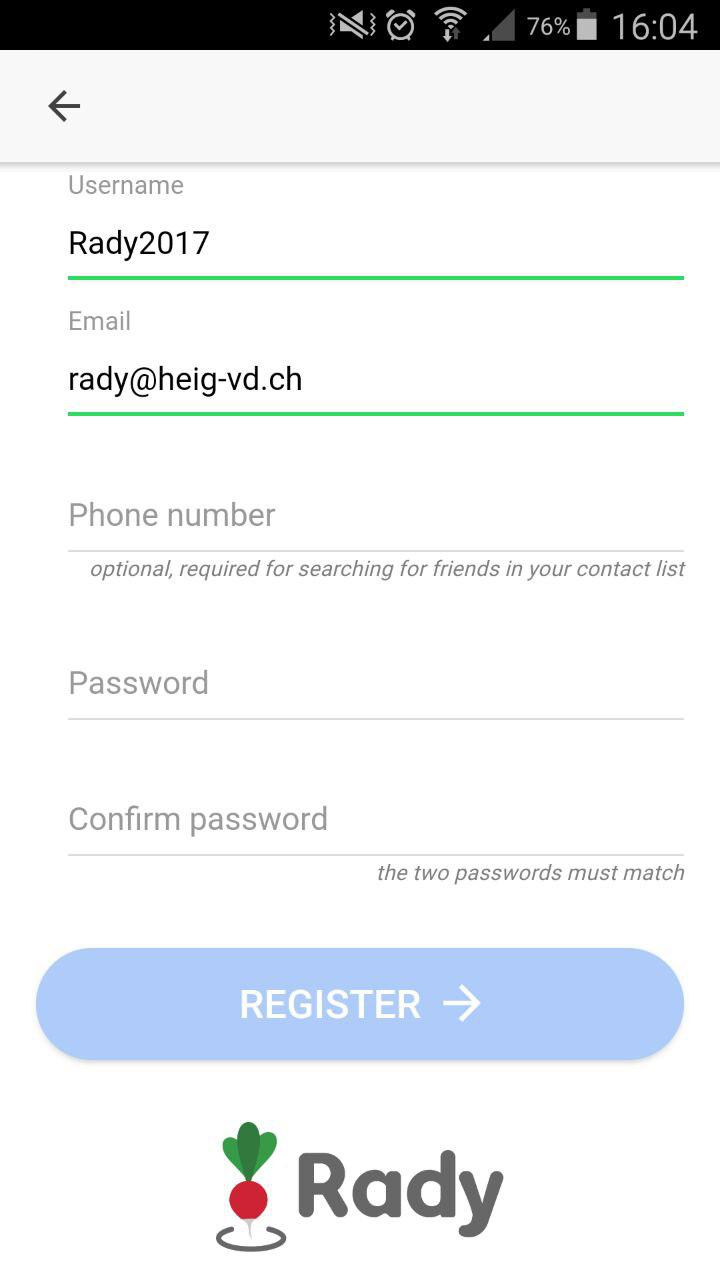
\includegraphics[scale=0.4]{../screenshot/screenshot-register2}
		\caption{Register}
		\label{Register}
	\end{figure} 
	Cette écran vous premet de vous enregistrer sur l'application si vous ne possédez pas encore de compte. Pour ce faire veuillez simplement remplire tous les différents champs du formulaire en prenant soin d'entrer des informations valides.
	
	\subsection{Forgot password}
	\begin{figure}[H]
		\centering
		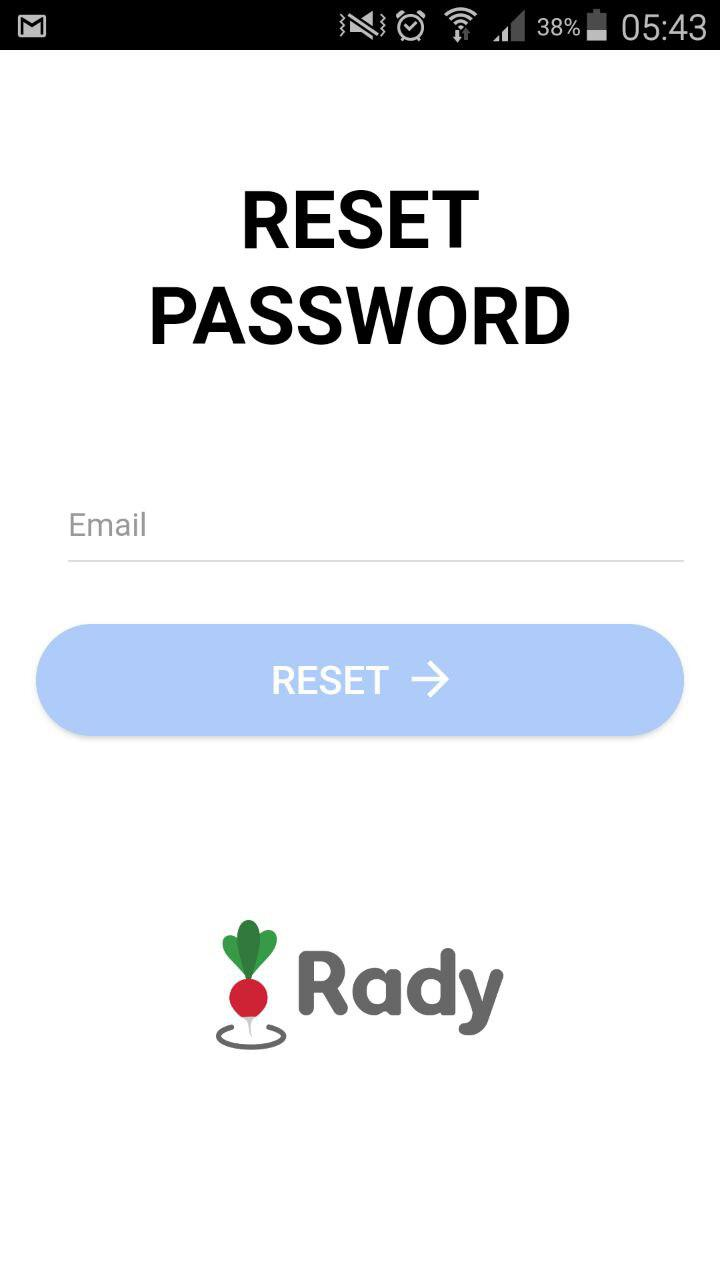
\includegraphics[scale=0.4]{../screenshot/screenshot-reset-password}
		\caption{Forgot password}
		\label{Forgot password}
	\end{figure} 
	
	Sur cette page vous récupérerez votre mot de passe en inscrivant simplement votre e-mail dans le champ prévu à cet effet. Un e-mail vous sera envoyé avec les instructions nécessaire pour votre prochaine reconnexion.
	
	\subsection{Contact-list}
	\begin{figure}[H]
		\centering
		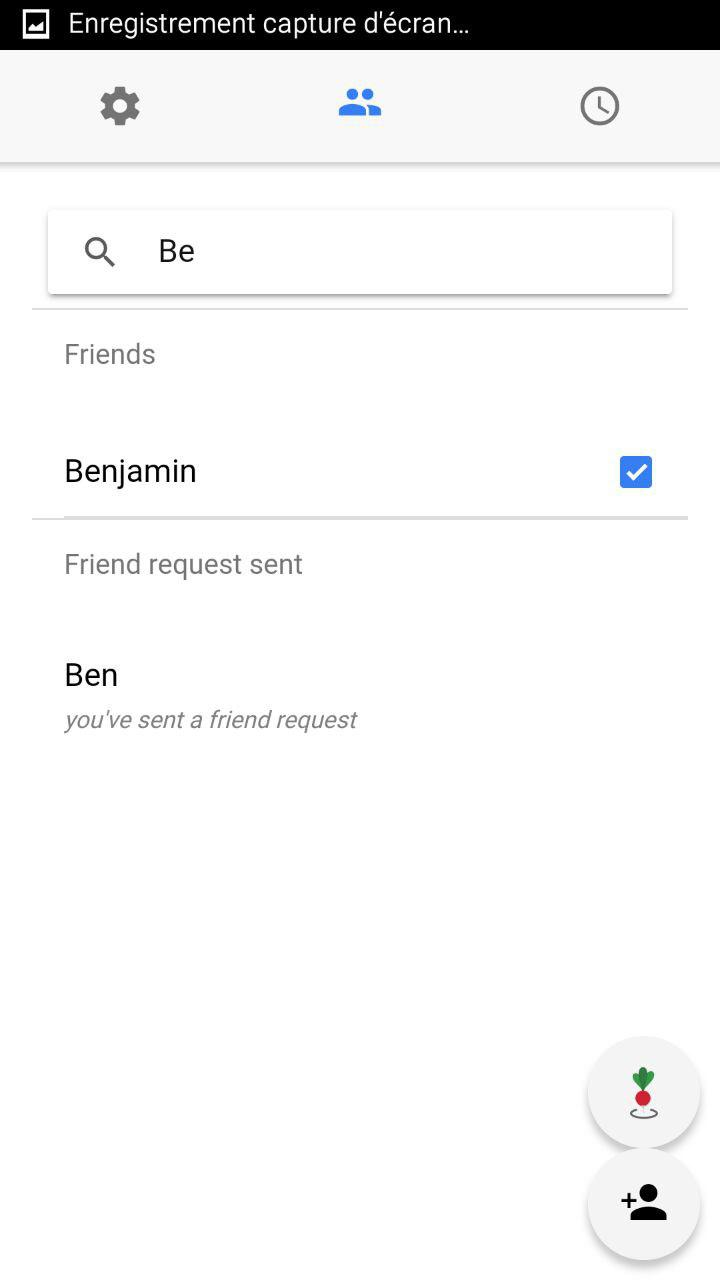
\includegraphics[scale=0.4]{../screenshot/screenshot-contact-list2}
		\caption{Contact-list}
		\label{Contact-list}
	\end{figure} 
	Cette page est la page d'arrivé après l'authentification. Elle donne accès à l'ajout de contact via l'icône avec un "+", et aux différents onglets de tabulation "paramètres" et "historique". Sur cette interface vous trouverez aussi un champ de recherche permettant de filtrer vos contacts.
	
	\subsection{History}
	\begin{figure}[H]
		\centering
		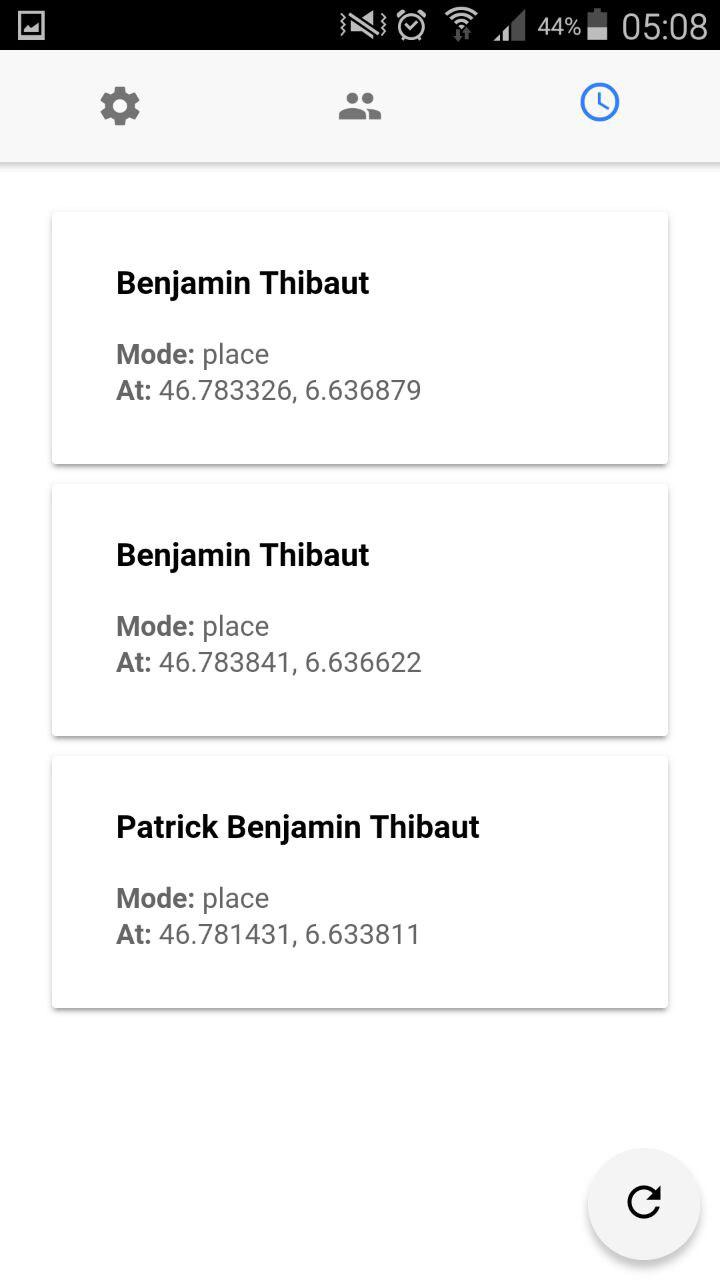
\includegraphics[scale=0.4]{../screenshot/screenshot-history}
		\caption{History}
		\label{History}
	\end{figure} 
	Vous pouvez à présent revoir vos anciens rendez-vous. Si vous les selectionnez vous pourrez les relancer à nouveau.
	Vous disposez également d'un bouton situé en bas à droite de votre écran vous permettant de recharger votre historique.
	
	
	\subsection{Settings}
	\begin{figure}[H]
		\centering
		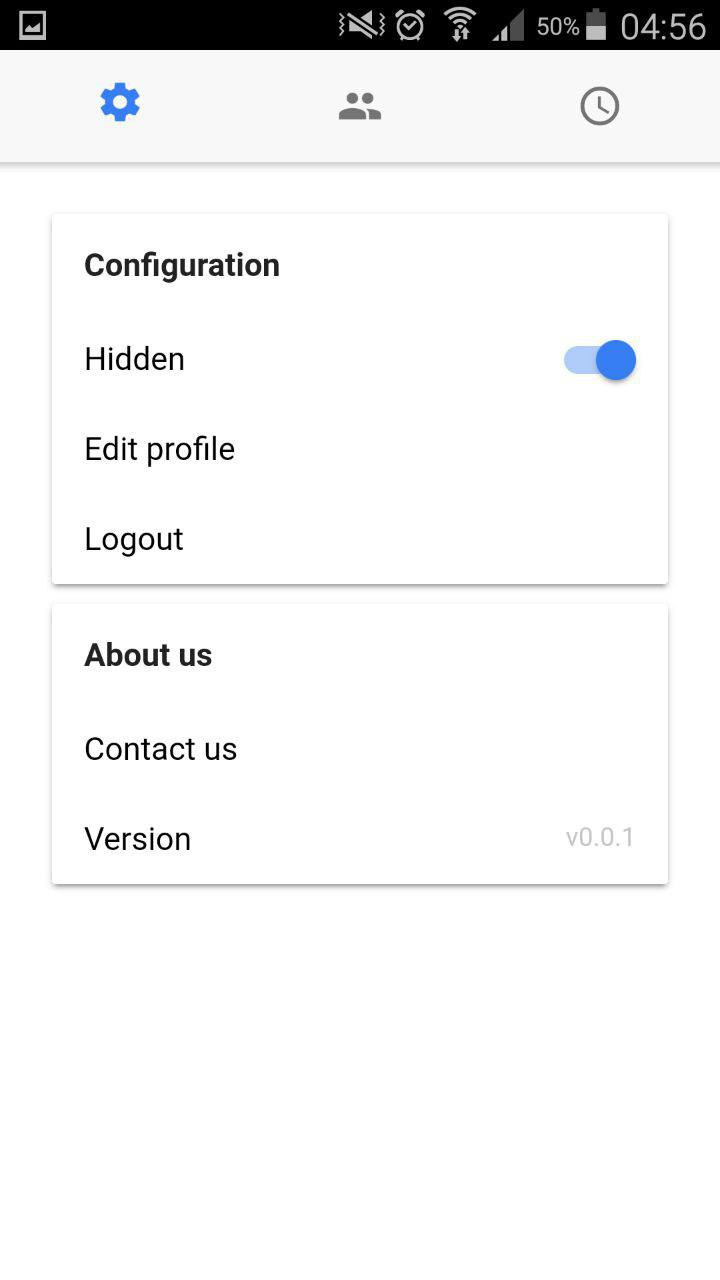
\includegraphics[scale=0.4]{../screenshot/screenshot-settings}
		\caption{Settings}
		\label{Settings}
	\end{figure} 
	Dans ce panneau vous avec accès aux différents paramètres et aux informations nous concernant. La bascule Hidden vous permet de vous mettre en mode invisible aupres de vos amis. Le bouton Edit profile vous permet de changer vos informations de profil et de les sauvegarder sur le serveur.
	Le bouton Logout vous donne accès à la fonction de déconnexion et vous ramène à l'écran d'authentification. Enfin le bouton Contact us vous permet de nous écrire en nous envoyant directement des messages.
	\subsection{Edit-profile}
		\begin{figure}[H]
			\centering
			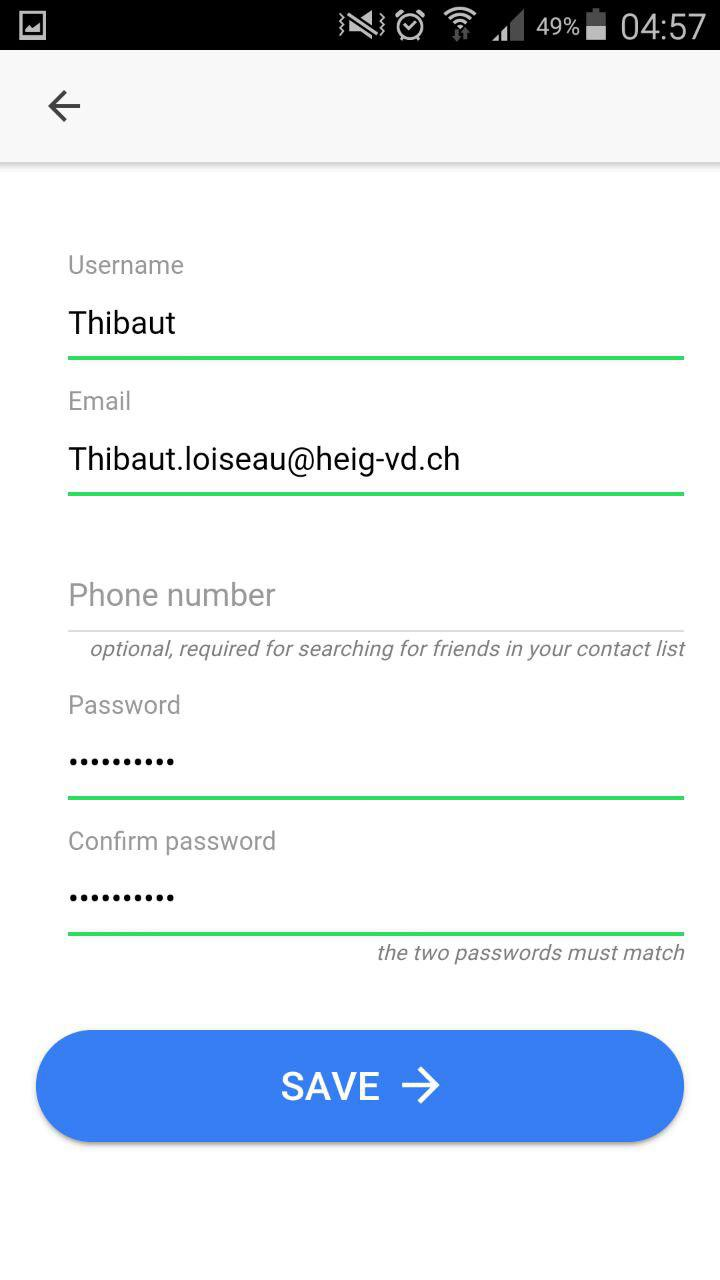
\includegraphics[scale=0.4]{../screenshot/screenshot-edit-profile}
			\caption{Edit-profile}
			\label{Edit-profile}
		\end{figure} 
	Dans cet écran tous les champs modifié avant l'appuie sur le bouton save seront enregistré et envoyé sur le serveur.
	\subsection{Add-contact}
		\begin{figure}[H]
			\centering
			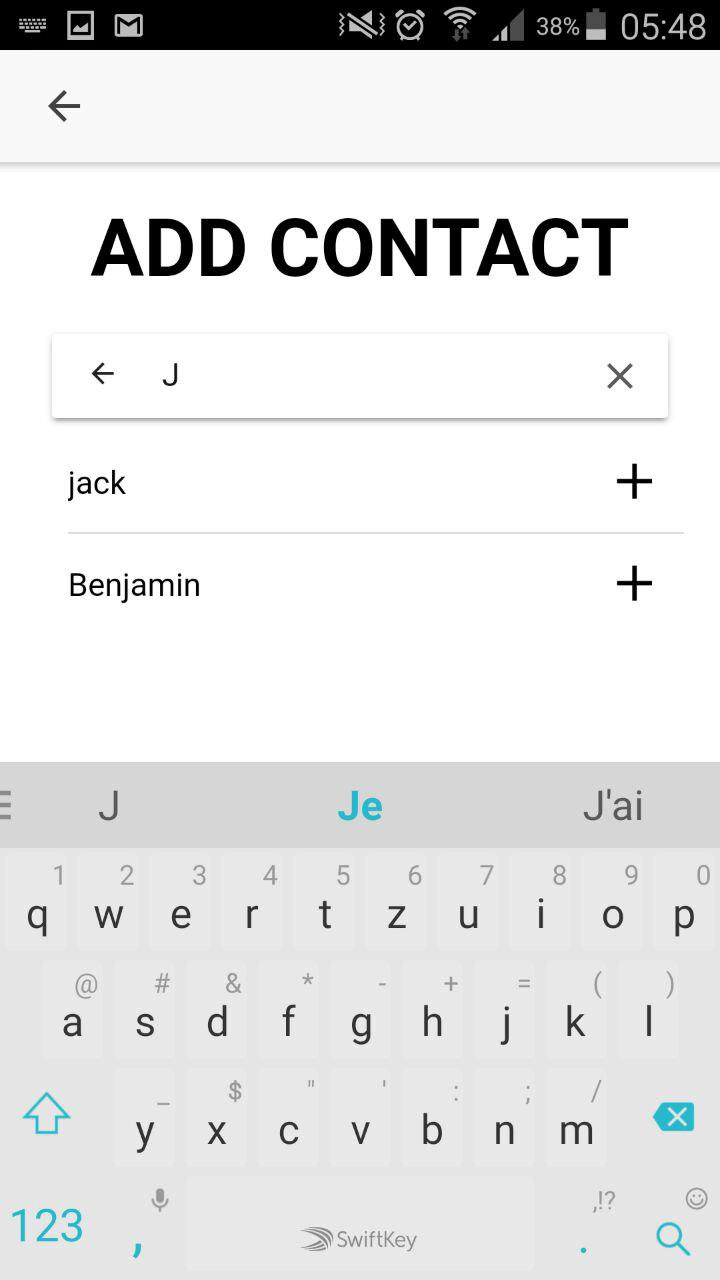
\includegraphics[scale=0.4]{../screenshot/screenshot-add-contact}
			\caption{Add-contact}
			\label{Add-contact}
		\end{figure} 
	Dans cette interface il vous suffit de rentrer le pseudo ou une partie du pseudo de la personne recherché pour que celle ci s'affiche. Dès son apparition vous pouvez en cliquant sur le "+" l'inviter à devenir votre ami.
	\subsection{Gathering}
	\begin{figure}[H]
		\centering
		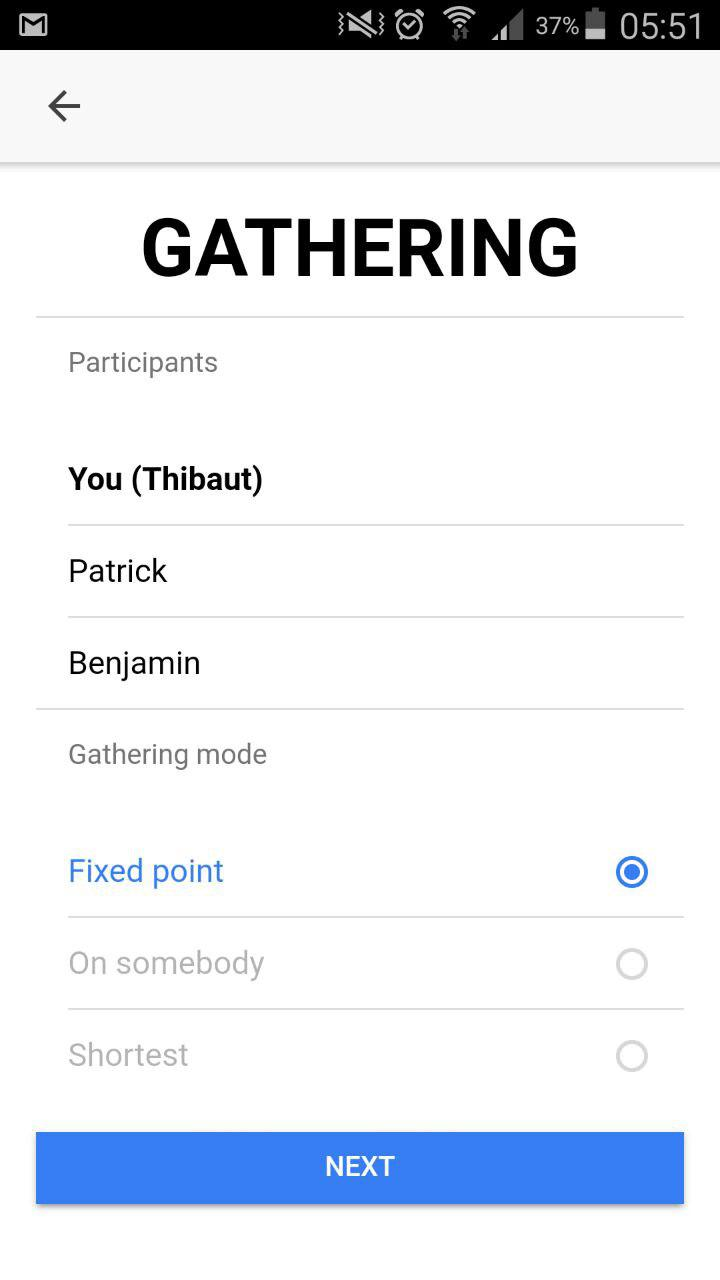
\includegraphics[scale=0.4]{../screenshot/screenshot-gathering-init}
		\caption{Gathering-initialisation}
		\label{Gathering-initialisation}
	\end{figure} 
	Vous voici à présent sur la page d'initialisation de la rencontre. Sur cette page vous pouvez choisir le mode de rencontre souhaité. Avant de passé à l'interface suivante.
	\begin{figure}[H]
		\centering
		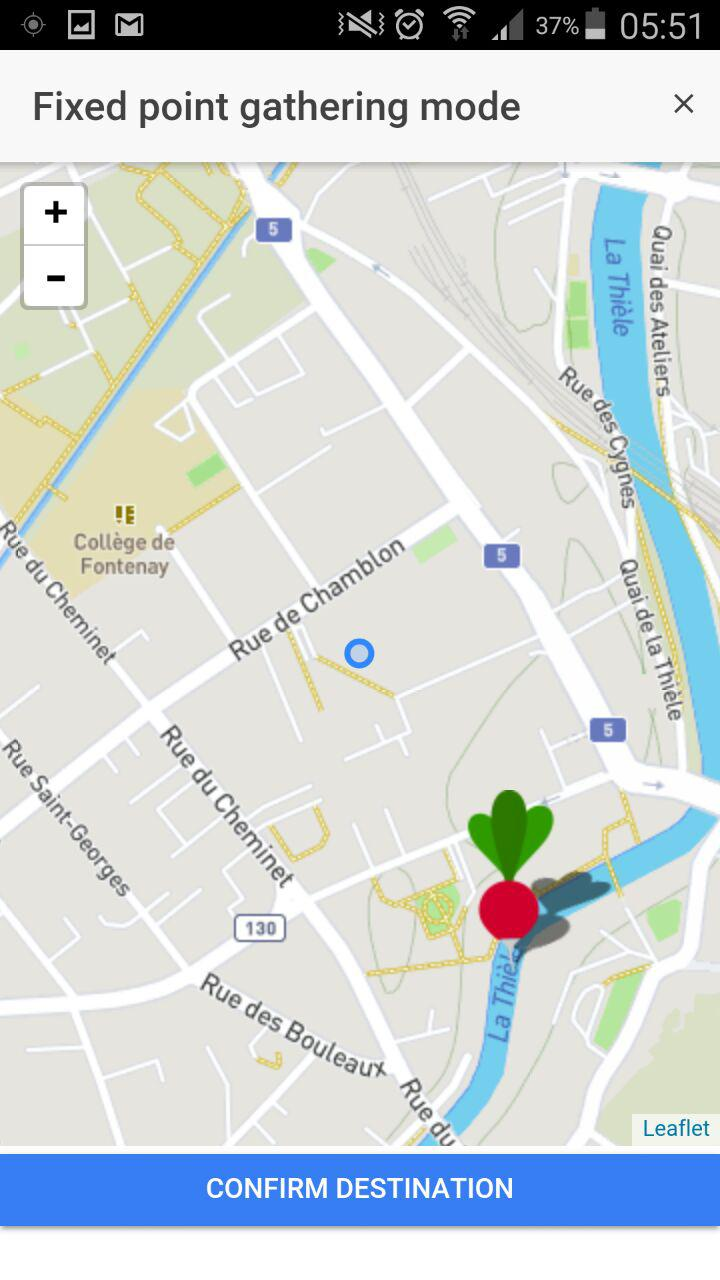
\includegraphics{../screenshot/screenshot-gathering-add-point}
		\caption{Gathering add point}
		\label{Gathering add point}
	\end{figure} 
	Si vous avez choisi le mode point fixe, vous êtes donc invité à placer un marqueur sur la carte prévu à cet effet. Ce marqueur servira de point de destination à tous les membres de la réunion. Une fois cette action effectué vous pouvez cliquer sur le bouton de confirmation afin de transmettre les invitations à tous les membres.
	\begin{figure}[H]
		\centering
		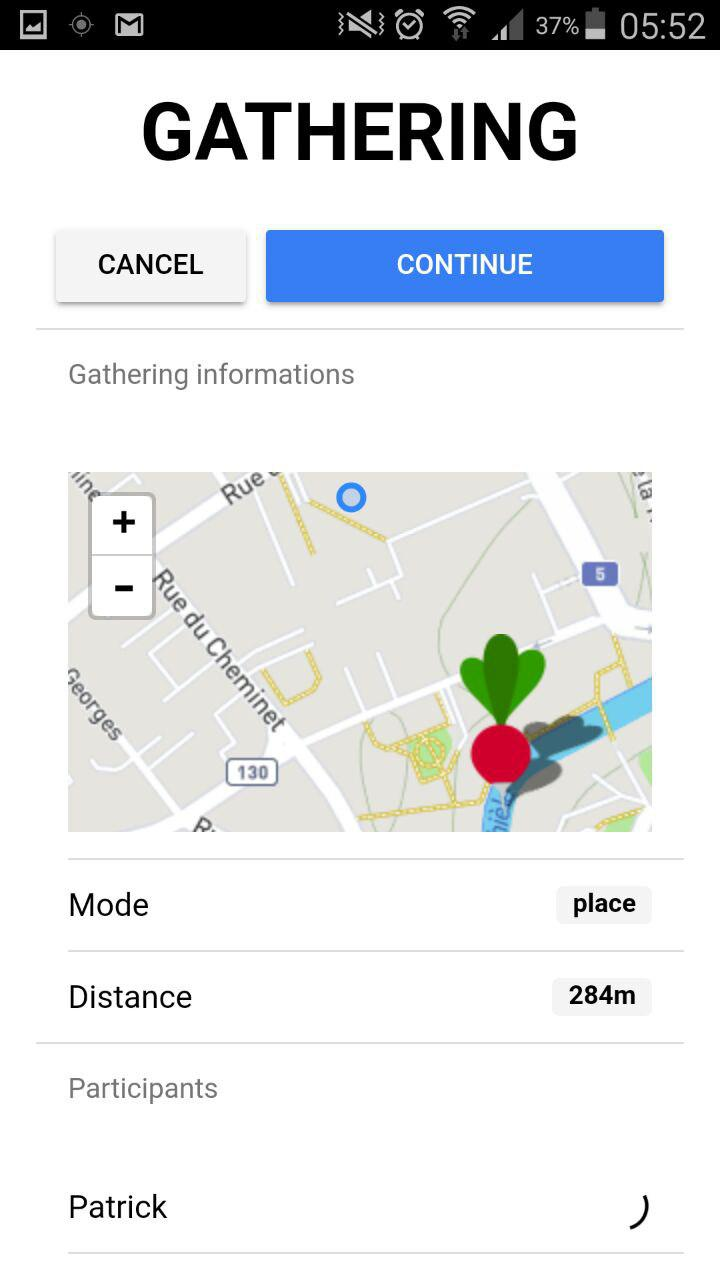
\includegraphics[scale=0.4]{../screenshot/screenshot-gathering-start}
		\caption{Gathering start}
		\label{Gathering start}
	\end{figure} 
	Arrivé sur cet écran vous pouvez soit anuler la réunion soit décider de continuer. Si vous le faite votre téléphone se transformera en véritable carte muni d'une boussole vous indiquant non pas le nord mais le cap à suivre pour arriver à votre destination.
	\begin{figure}[H]
		\centering
		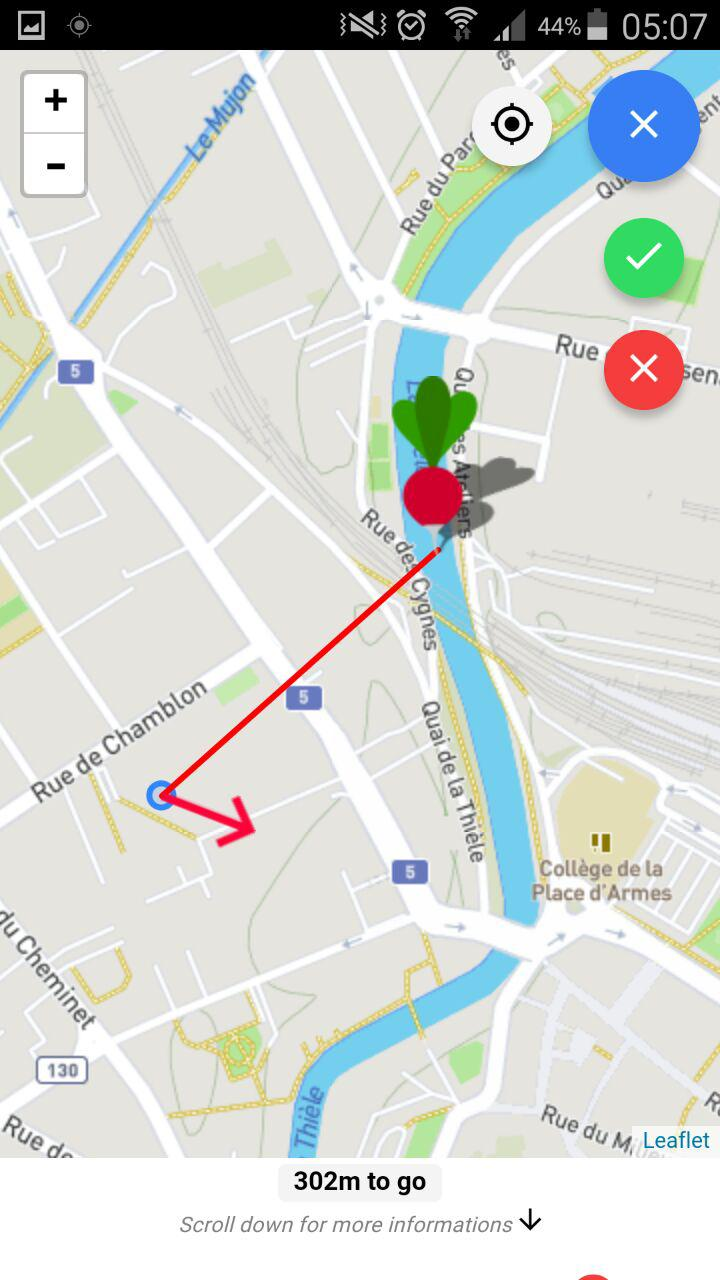
\includegraphics{../screenshot/screenshot-map}
		\caption{Gathering map}
		\label{Gathering map}
	\end{figure} 
	Sur ce dernier écran vous pouvez recentrer la carte sur votre position à l'aide de l'icone cible ou bien quitter le rendez-vous à l'aide de la croix ou encore signaler à tous les autres membres concerné que vous avez bien atteint votre destination.
		
	

\end{document}
